\chapter{Continuous Normalizing Flows}
\label{chapter:cnf}

\section{Introduction to Normalizing Flows}
\label{section:cnf:normalizing_flows}

\osc{What section?}
Section ends with a question: "What if we can start with a simple distribution and distort it into a more complex one?". To answer this question, let us first examine what happens with \osc{happens to} the densities as we transform some random variable.

Let $ x \in R^d $ be a random variable with an underlying probability density function $ P_x $ and $ f: R^d \mapsto R^d $ be an invertible transformation. Then, if

\begin{displaymath}
    y = f(x),
\end{displaymath}

\osc{why not $P_X(x)$ and $P_Y(y)$?}

i.e. we obtain the random variable $ y $ by transforming $ x $ using $ f $, the probability density function $ P_y $ of $ y $ can be obtained using the change of variables formula

\osc{$\det$ not $det$}

\begin{equation}
    \label{equation:cnf:nf:change_density}
    P_y(y) = P_x(x) \left | det \frac{\partial f}{\partial x} \right |^{-1}
\end{equation}

and the change in log density becomes

\begin{equation}
    \label{equation:cnf:nf:change_log_density}
    \log P_y(y) = \log P_x(x) - \log \left | det \frac{\partial f}{\partial x} \right |.
\end{equation}

Now let us assume that instead of a single transformation, we want to apply a series of transformations. Let $ f_i: R^d \mapsto R^d, \ i \in \{1, \ ..., \ n\} $ be $ n $ different transformations, and let $ z_0 $ be an initial random variable with a probability density function $ P_{z_0} $. Then, we can denote the composition of functions $ f_i $ on $ z_0 $ as

\begin{displaymath}
    z_n = f_n \circ ... \circ f_1(z_0),
\end{displaymath}

with the probability density function of $ z_n $ being

\begin{equation}
    \label{equation:cnf:nf:total_change_density}
    P_{z_n}(z_n) = P_{z_0}(z_0) \prod_{i=1}^n \left | det \frac{\partial f_i}{\partial z_{i-1}} \right |^{-1}
\end{equation}

and the total change in log density being

\begin{equation}
    \label{equation:cnf:nf:total_change_log_density}
    \log P_{z_n}(z_n) = \log P_{z_0}(z_0) - \sum_{i=1}^n \log \left | det \frac{\partial f_i}{\partial z_{i-1}} \right |.
\end{equation}

This technique is called a normalizing flow and was formalized by \citet{rezende2015variational}. They start with a simple probability density function and transform it into a more complex one, by applying a sequence of invertible transformations until a desired level of complexity is obtained. Some simple normalizing flows introduced in their paper \citep{rezende2015variational} are the \emph{planar} and the \emph{radial} flow. The transformation for the planar flow is

\begin{displaymath}
    f(z) = z + uh(w^Tz + b),
\end{displaymath}

where $ u, w \in R^d, b \in R $ and $ h $ is a smooth element-wise non-linearity. On the other hand, the transformation of the radial flow is

\begin{displaymath}
    f(z) = z + \beta h(\alpha, r)(z - z_0),
\end{displaymath}

where $ z_0 \in R^d, \ \alpha \in R^+, \ \beta \in R, \ r = \lvert z - z_0 \rvert $ and $ h(\alpha, \ r) = \nicefrac{1}{\alpha + r} $. The planar flow introduces hyperplanes into the space, and the radial flow introduces spheres into the space.

\begin{figure}[ht]
      \centering
      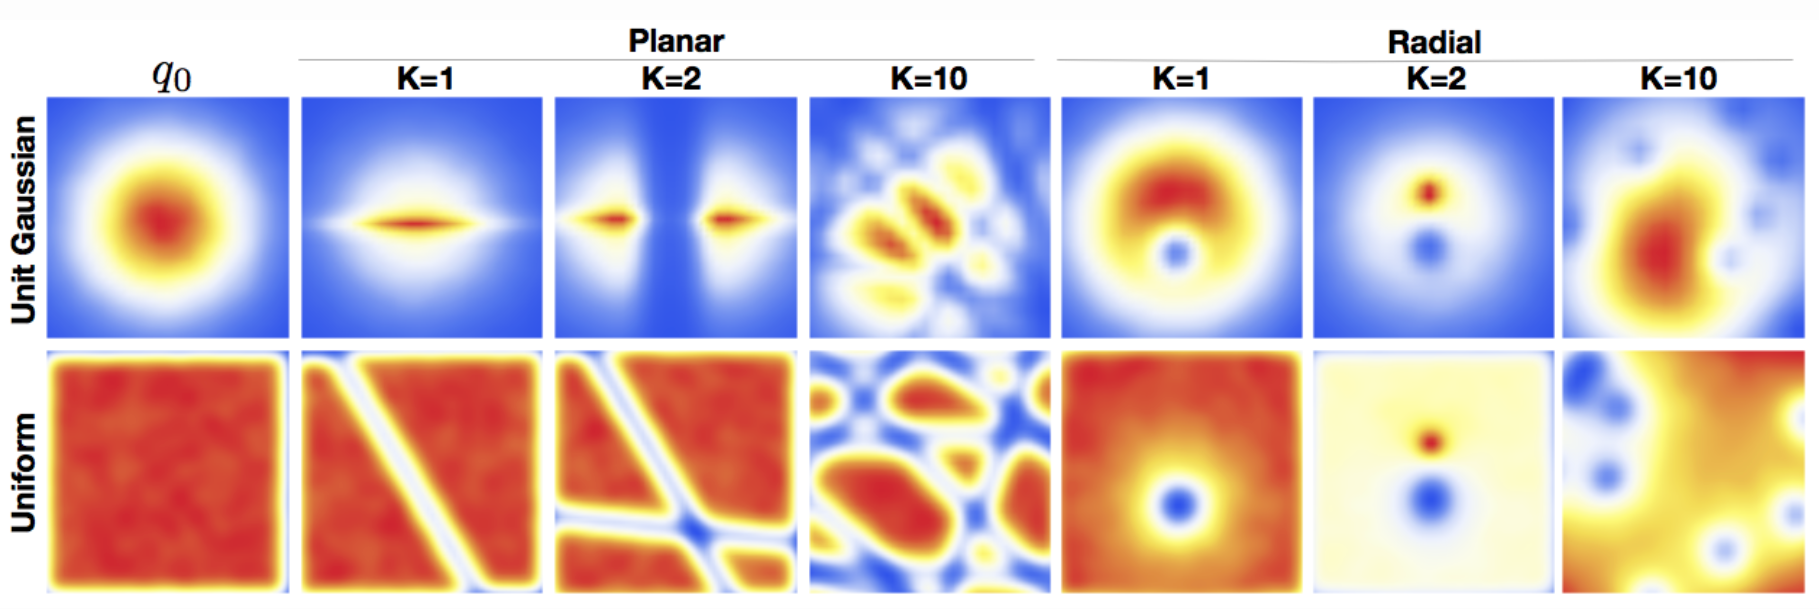
\includegraphics[width=\columnwidth]{figures/planar_radial_flows.png}
      \caption{The effect of planar and radial flows on uniform and unit Gaussian distributions \citep{rezende2015variational}.}
      \label{figure:cnf:planar_radial_flows}
\end{figure}

However, in practice, normalizing flows are limited due to their high computational complexity. By looking at equations \ref{equation:cnf:nf:change_density} up to \ref{equation:cnf:nf:total_change_log_density}, we can deduce that normalizing flows require calculating a determinant, which is generally a $ \mathcal{O}(d^3) $ operation. Therefore, their expressiveness is limited by the need to use relatively simple transformations, which Jacobians are easy to compute. For example, both the planar and radial flow allow for linear cost determinant computation and their effect are illustrated on figure \ref{figure:cnf:planar_radial_flows}.

\section{Continuous Normalizing Flows}
\label{section:cnf:cnf}

The previous chapter introduces a novel family of neural models under the name NeuralODEs. \citet{chen2018neural} noticed that the discretized equation \ref{equation:ode:resnet} also appears in Normalizing Flows \citep{rezende2015variational} and the NICE framework \citep{dinh2014nice}. They further realized that performing continuous transformations has an unexpected side effect to the change of variables formula.

\begin{figure}[ht]
      \centering
      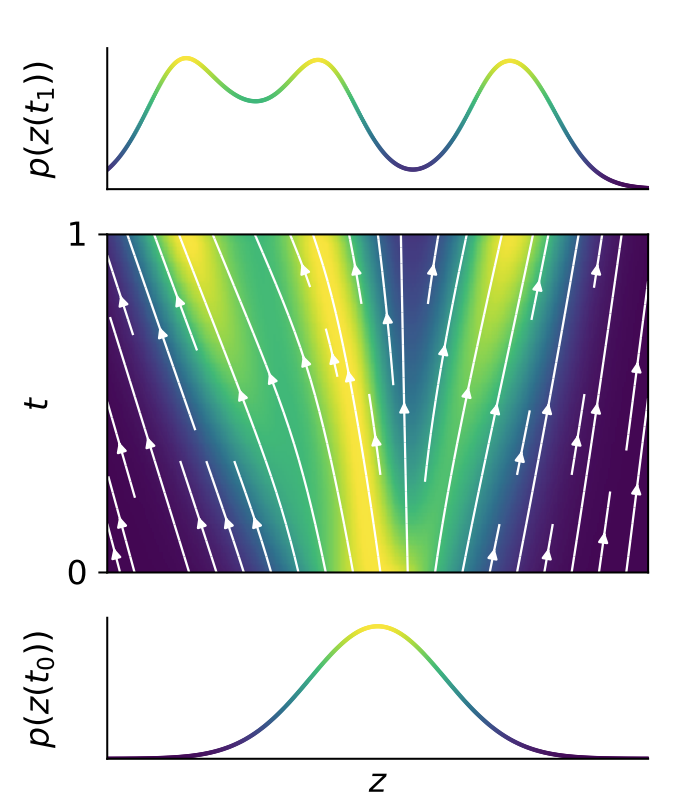
\includegraphics[width=0.5\columnwidth]{figures/cnf_transformations.png}
      \caption{Continuous Normalizing Flows distorting a single mode Gaussian into a more complex distribution \citep{grathwohl2018ffjord}}
      \label{figure:cnf:cnf_transformations}
\end{figure}

Recall from equation \ref{equation:cnf:nf:change_log_density}, that when applying discrete transformations, the change in log density is given by

\begin{align}
    z_{1} &= f(z_{0}), \\
    \log p(z_{1}) &= \log p(z_{0}) - \log \left \lvert det \frac{\partial f}{\partial z_{0}} \right \rvert,
\end{align}

however, when going into the continuous domain, the change in log density becomes

\begin{align}
    \frac{\partial z(t)}{\partial t} &= f(z(t), t), \\
    \frac {\partial \log p(z(t))} {\partial t} &= -Tr \left( \frac{\partial f}{\partial z(t)} \right),
\end{align}

with the total change in log density given by

\begin{displaymath}
    \log p(z(t_1)) = \log p(z(t_0)) - \int_{t_0}^{t_1} Tr \left( \frac{\partial f}{\partial z(t)} \right) dt    
\end{displaymath}

This combination of NeuralODEs and Normalizing Flows is called \emph{Continuous Normalizing Flows (CNFs)} and can be visualized on Figure \ref{figure:cnf:cnfs_visualization}. One huge difference in the continuous case, is that instead of computing the determinant of the Jacobian, we only need to calculate the trace. Determinants are generally calculated in $ \mathcal{O}(d^3) $, however, the trace is a linear cost operation.

\begin{figure}[ht]
      \centering
      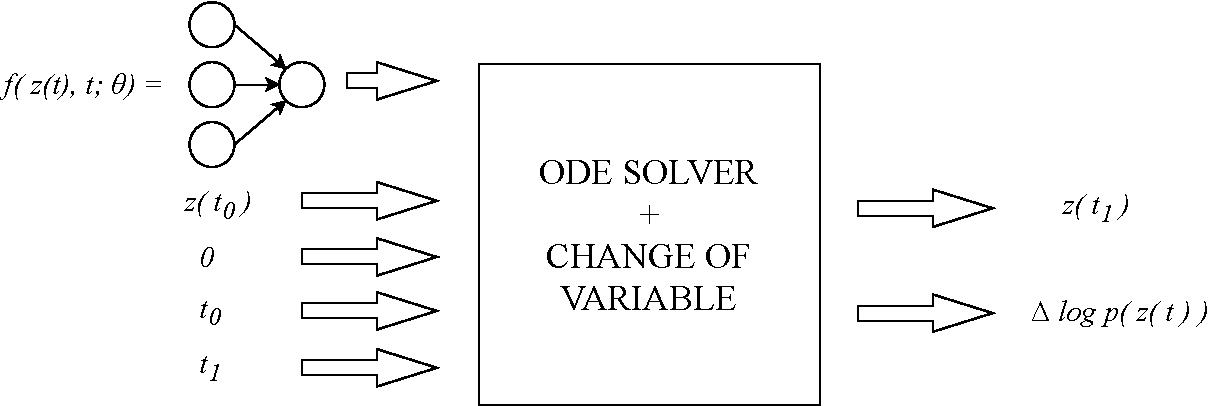
\includegraphics[width=\columnwidth]{figures/cnfs_visualization.pdf}
      \caption{$f(z(t), \ t; \ \theta) $ is neural network specifying the differential equation, $ z(t_0) $ is the initial state, $ 0 $ is the initial log-density, $ t_0 $ is the initial time, $ t_1 $ is the final time, $ z(t_1) $ is the final state and $ \Delta \log p(z(t)) $ is the change in log-density.}
      \label{figure:cnf:cnfs_visualization}
\end{figure}

Unfortunately, the overall complexity of the method above is still $ \mathcal{O}(d^2) $ due to the Jacobian, which even though better, is still restrictive. \citet{grathwohl2018ffjord} further optimize the above method and reduce the overall complexity to $ \mathcal{O}(d) $. They achieve this in two steps. First, Vector-Jacobian products can be computed efficiently using reverse-mode automatic differentiation. Secondly, they show that they can get unbiased estimates of the trace of the Jacobian, by using the Hutchinson’s trace estimator \citep{hutchinson1990stochastic}. Consequently, they claim that Continuous Normalizing Flows implemented in this fashion can be considered unrestricted due to the free-form Jacobian of the transformation $ f $.

\osc{don't put spaces before footnotes, and put all urls into \url{https://example.com/}}

\citet{grathwohl2018ffjord} additionally provide a PyTorch framework \footnote{https://github.com/rtqichen/ffjord/} with the previously mentioned improvements. Within their framework we can apply CNFs to random variables and log densities as

\begin{displaymath}
    \underbrace{
        \begin{matrix}
            \begin{bmatrix}
                z(t_1) \\
                \Delta \log p(z_t) %\log p(z_{t_1}) - \log p(z_{t_0})
            \end{bmatrix}
        \end{matrix}
    }_{Solution}
    =
        \bigintss_{t_0}^{t_1}
        \underbrace{
            \begin{matrix}
                \begin{bmatrix}
                    f(z(t), t; \theta) \\
                    Tr \left ( \frac{\partial f}{\partial z(t)} \right)
                \end{bmatrix}
            \end{matrix}
    }_{Dynamics}
    dt = cnf
    \Bigg (
        \underbrace{
            \begin{matrix}
                \begin{bmatrix}
                    z(t_0) \\
                    0
                \end{bmatrix}
            \end{matrix},
        }_{Initial Values}
        t_0, \ t_1, \ f
    \Bigg )
\end{displaymath}

and finally we can obtain $ \log p(z_{t_1}) $  as 

\begin{displaymath}
    \log p(z_{t_1}) = \log p(z_{t_0}) - \Delta \log p(z_t).
\end{displaymath}
